\section{Results}
\label{sec:results}

% Generated by scripts/paper_tables.py. Do not edit.
\begin{table*}[t]
\centering
\footnotesize
\setlength{\tabcolsep}{3pt}
\TabCaption{tab:bench}{Test ROC-AUC under every protocol}{LR: logistic regression; EBM-A, EBM-P: additive EBM and EBM with pairwise terms. Random: five stratified splits. Time: last 15\% of tasks by start time; Known/New: test tasks whose user does or does not appear in training. Grouped: five user-grouped folds. $-$U1, $-$U1,4: random split without User~1, or Users~1 and~4. Bold: best in the column of each panel. $^{\circ}$: not significantly different from \kaam{} (paired bootstrap over test tasks, over users for Grouped; Holm). Under the protocols the EBMs were fitted on the original sample only.}
\begin{tabular}{@{}lccccccc@{}}
\toprule
Model & Random & Time & Known & New & Grouped & $-$U1 & $-$U1,4 \\
\midrule
\multicolumn{8}{@{}l}{\emph{Full trace (\V{data.full.tasks} tasks)}} \\
KAAM & 0.766 & 0.594 & 0.596 & 0.466 & \textbf{0.641} & 0.703 & 0.672 \\
LR & 0.732 & 0.576 & 0.580 & 0.462$^{\circ}$ & 0.600 & 0.656 & 0.630 \\
MLP & 0.804 & 0.596$^{\circ}$ & \textbf{0.599}$^{\circ}$ & 0.482$^{\circ}$ & 0.637$^{\circ}$ & 0.721 & 0.698 \\
LightGBM & \textbf{0.900} & \textbf{0.599}$^{\circ}$ & \textbf{0.599}$^{\circ}$ & \textbf{0.534} & 0.566$^{\circ}$ & \textbf{0.845} & \textbf{0.805} \\
\midrule
\multicolumn{8}{@{}l}{\emph{Original sample (\V{data.orig.tasks} tasks)}} \\
KAAM & 0.744 & 0.595 & 0.603 & 0.515 & \textbf{0.620} & 0.698 & 0.627 \\
LR & 0.723 & 0.588$^{\circ}$ & 0.589$^{\circ}$ & \textbf{0.565}$^{\circ}$ & 0.561$^{\circ}$ & 0.662 & 0.602 \\
MLP & 0.722 & 0.523 & 0.533 & 0.548$^{\circ}$ & 0.540 & 0.681$^{\circ}$ & 0.531 \\
LightGBM & \textbf{0.810} & \textbf{0.619}$^{\circ}$ & \textbf{0.620}$^{\circ}$ & 0.552$^{\circ}$ & 0.502$^{\circ}$ & \textbf{0.756} & 0.673 \\
EBM-A & 0.756 & 0.595$^{\circ}$ & 0.596$^{\circ}$ & 0.533$^{\circ}$ & 0.489$^{\circ}$ & 0.722 & 0.646 \\
EBM-P & 0.803 & 0.573$^{\circ}$ & 0.565$^{\circ}$ & 0.539$^{\circ}$ & 0.504$^{\circ}$ & 0.752 & \textbf{0.685} \\
\bottomrule
\end{tabular}
\TabNotes
\end{table*}


Table~\ref{tab:bench} gives the test ROC-AUC of every model under every protocol.

\emph{Random splits.} On the full trace \kaam{} (\V{full.random.kaam.auc}) is above logistic regression (\V{full.random.lr.diff}) and below the MLP (\V{full.random.mlp.diff}) and LightGBM (\V{full.random.lgbm.diff}). On the original sample, where all six models were fitted, the two additive models (\kaam{} \V{orig.random.kaam.auc}, EBM-A \V{orig.random.ebm.auc}) are close, and so are the two models with interactions (LightGBM \V{orig.random.lgbm.auc}, EBM-P \V{orig.random.ebmi.auc}). All differences from \kaam{} are significant after Holm correction, so \kaam{} matches none of the baselines; the additive EBM fitted once on the full trace's canonical split reaches \V{full.s42.ebm.auc} against \V{full.s42.kaam.auc} for \kaam{}. In each random split of the full trace \V{rf.full.dup.random.min} to \V{rf.full.dup.random.max} of the test tasks have an exact copy of all ten features in training (\V{rf.full.dup.time.max} in the time-ordered split, \V{rf.full.dup.grouped.min} to \V{rf.full.dup.grouped.max} in the grouped folds), so a random split rewards recognising duplicated requests: on the canonical split a lookup of identical training tasks scores \V{ph.full.dup.s42.lookup} on the duplicated test tasks, and LightGBM scores \V{ph.full.dup.s42.lgbm.dup} on them against \V{ph.full.dup.s42.lgbm.nondup} on the rest. Resampling whole users instead of tasks widens the intervals, and the three full-trace differences stay significant (Holm-adjusted $p$ = \V{ph.full.cb.random.lgbm.p} for LightGBM). Under this protocol LightGBM, the MLP and \kaam{} are close to calibrated (ECE at most \V{full.random.kaam.ece}).

\emph{Time-ordered split.} On the last \V{prot.time.test} of the trace every model scores between \V{full.time.minauc} and \V{full.time.maxauc}. Users seen in training make up \V{full.split.time.t.knownshare} of the test tasks, and on them the scores lie between \V{full.timeknown.minauc} and \V{full.timeknown.maxauc}. The validation period before it is a burst dominated by User~1 (\V{rf.full.time.val.u1} of its tasks; failure rate \V{full.split.time.t.rateval}, \V{rf.full.time.val.rateno1} without User~1), on which the models reached \V{full.time.minvalauc} to \V{full.time.maxvalauc}, so selection on it overstated test accuracy; the test week starts \V{rf.full.time.gap} days after the last training task. On the \V{full.split.time.t.newn} new-user test tasks, from \V{rf.full.time.newusers} users, LightGBM is best (\V{full.timenew.lgbm.auc} against \V{full.timenew.kaam.auc} for \kaam{}), a difference that is \V{full.timenew.lgbm.sig} under a task-level bootstrap and \V{ph.full.cb.timenew.lgbm.sig} when whole users are resampled (\V{ph.full.cb.timenew.lgbm.dci}).

\emph{User-grouped folds.} StratifiedGroupKFold places User~1 with two small users in fold~\V{full.mech.u1fold} (\V{full.mech.u1.ntest} test tasks from \V{full.mech.u1.testusers} users), in effect a test on User~1 alone; the other folds hold \V{full.mech.nou.min.users} to \V{full.mech.nou.max.users} test users each. On those folds the mean AUCs are \V{full.gnou.mlp.auc} (MLP), \V{full.gnou.kaam.auc} (\kaam{}), \V{full.gnou.lr.auc} (LR) and \V{full.gnou.lgbm.auc} (LightGBM); over all five folds \kaam{} has the highest mean (\V{full.grouped.kaam.auc}), but not significantly above the MLP or LightGBM, so no model is clearly best on new users (Fig.~\ref{fig:folds}). Resampling users within the four folds without User~1, \kaam{}'s differences from the MLP, LR and LightGBM are \V{ph.full.gnou.mlp.sig} (Holm-adjusted $p$ = \V{ph.full.gnou.mlp.p}, \V{ph.full.gnou.lr.p} and \V{ph.full.gnou.lgbm.p}). LightGBM's grouped fits stopped after \V{full.lgbm.grouped.minrounds} to \V{full.lgbm.grouped.maxrounds} boosting rounds on average, against \V{full.lgbm.random.minrounds} to \V{full.lgbm.random.maxrounds} on random splits, so its low grouped score reflects ensembles cut almost at once by early stopping on validation users. The one-core rule is the clearest mechanism: with User~1 in training, one-core tasks fail at \V{rf.oc.with.minone} to \V{rf.oc.with.maxone} against about \V{rf.oc.with.minother} for other tasks, and User~1 holds \V{rf.oc.with.minu1} to \V{rf.oc.with.maxu1} of them; without User~1 they fail at \V{rf.oc.groupedf4.one} against \V{rf.oc.groupedf4.other}. Among held-out users, ranking by $-$\feat{plan_cpu} gives \V{full.mech.nou.min.teauc} to \V{full.mech.nou.max.teauc}, below chance in \V{full.mech.nou.nrev} of the four many-user folds.

\begin{figure}[t]
\centering
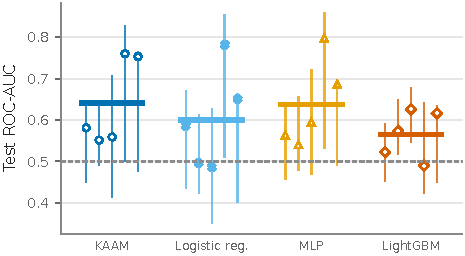
\includegraphics[width=0.92\linewidth]{figures/grouped_folds.pdf}
\caption{User-grouped folds, full trace: AUC per fold with user-level 95\% intervals (markers) and the fold mean (bar). Dashed: chance.}
\label{fig:folds}
\end{figure}

\emph{Leaving out the dominant users.} Removing User~1 changes the test population (User~1's tasks fail at \V{users.full.u1.rate} against \V{users.full.nonu1.rate} for the others), so these AUCs are not comparable with the random protocol's. A post hoc like-for-like check scores the canonical models on the test tasks of the canonical split without User~1: \kaam{} reaches \V{ph.full.likea.kaam.auc} and LightGBM \V{ph.full.likea.lgbm.auc}. Trained without User~1 and tested on another draw from that population, \kaam{} gains \V{ph.full.likea.kaam.gain} and LR \V{ph.full.likea.lr.gain}, while LightGBM changes by \V{ph.full.likea.lgbm.gain}, so rules learned from User~1 cost the two models without interactions accuracy on other users. Without Users~1 and~4 LightGBM still leads \kaam{} by \V{full.louob.lgbm.absdiff}: its random-split lead is not explained by the dominant users, and exact duplicates (\V{rf.full.dup.louo.min} to \V{rf.full.dup.louo.max} of these test tasks) are one candidate.

\emph{Interpretability.} The centred \kaam{} contributions equal exact Kernel SHAP values to within \V{shap.maxdiff}. The \feat{plan_cpu} curve stands at \V{pc.randoms42.onecore} log-odds at one core on the canonical split and at \V{pc.louod1.onecore} with User~1 removed (Fig.~\ref{fig:plancpu}); the centred value also reflects each curve's overall shape, which changes from fit to fit. Validation chose no smoothness penalty on random splits and the strongest one on the time-ordered split and \V{full.lambda.grouped.em2} of five grouped folds. On the protocol's grid the median correlation of the shape functions of \kaam{} and the additive EBM is \V{ebm.r.median}, with close agreement on the telemetry curves and almost none on two discrete requests (\V{ebm.r.worstfeat}, $r=\V{ebm.r.min}$); at the training tasks' own values, an exploratory measure, the median is \V{ebm.rd.median}, so the two models differ mainly between observed request values\ifshowcurves{} (Fig.~\ref{fig:shapes})\fi. The curves are a complete account of each fitted model but not a stable account of the data: the \feat{plan_cpu} curve of the time-ordered split correlates \V{pc.timet.corr} with the canonical one.

\begin{figure}[t]
\centering
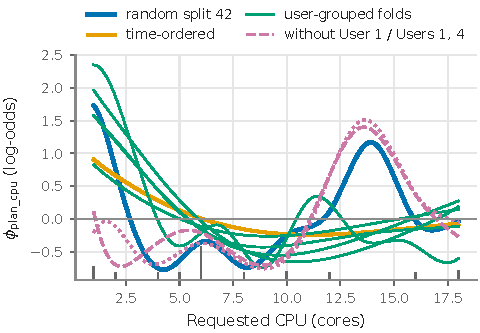
\includegraphics[width=0.92\linewidth]{figures/plan_cpu_protocols.pdf}
\caption{\kaam{}'s \feat{plan_cpu} curve under each protocol (full trace, seed~0), each centred on its mean over the canonical training 5th to 95th percentile of the request. Ticks: request values held by at least \V{fig.tickshare} of training tasks.}
\label{fig:plancpu}
\end{figure}

\ifshowcurves
\begin{figure}[t]
\centering
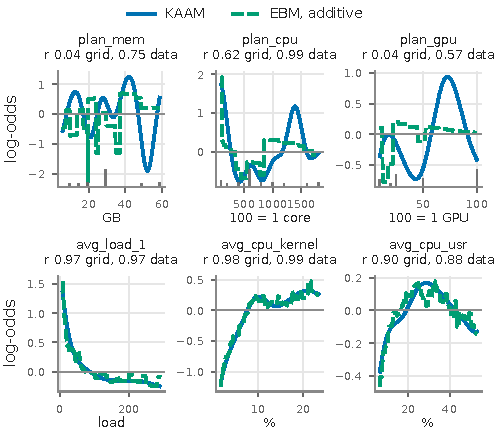
\includegraphics[width=\linewidth]{figures/shapes_kaam_ebm_ieee.pdf}
\caption{Shape functions of \kaam{} and the additive EBM on the canonical split for the three request features and the three telemetry features with the largest \kaam{} swing. Titles: correlation on the protocol's grid and, exploratory, at the training tasks' values.}
\label{fig:shapes}
\end{figure}
\fi

\emph{Case audits.} A rule fixed in the first version selects four test tasks of the canonical model: the most confident true positive and true negative, and the false negative and false positive with the highest risk at a threshold of 0.5. The most confident true positive (risk \V{case.tp.risk}) is a one-core request whose \feat{plan_cpu} term is \V{case.tp.c.plancpu}; its exact request occurs in \V{case.tp.samereq} training tasks, \V{case.tp.samerate} failed, \V{case.tp.sameu1} from User~1. The highest-risk false alarm (\V{case.fp.risk}) is another user's one-core task that receives the same term, although its own request failed in \V{case.fp.samerate} of \V{case.fp.samereq} training tasks\ifshowcase{} (Fig.~\ref{fig:waterfall})\fi.

\ifshowcase
\begin{figure*}[t]
\centering
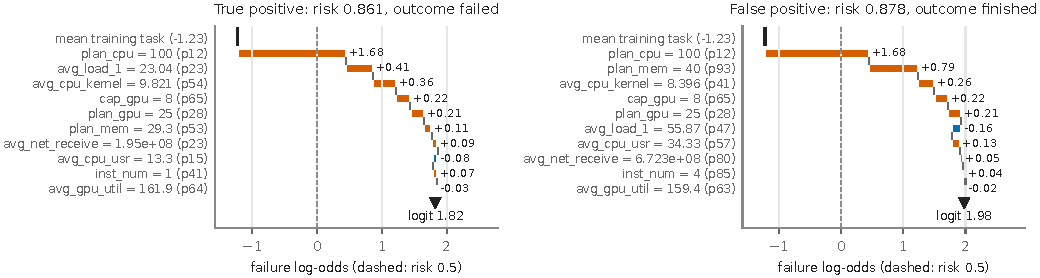
\includegraphics[width=\textwidth]{figures/case_waterfall_ieee.pdf}
\caption{Case audits of the canonical \kaam{}: from the logit of the mean training task (the bias plus each contribution's mean over training tasks) through the ten contributions, largest first, to the model's logit. Labels: raw value and its percentile among training tasks (pNN). Dashed: risk 0.5.}
\label{fig:waterfall}
\end{figure*}
\fi
